Оценку эффективности протоколов будем проводить по двум
параметрам:

\begin{itemize}
	\item коэффициент эффективности $k$ -- количество всех пакетов / количество переданных пакетов
	\item время от начала до конца передачи в секундах – $t$
\end{itemize}

Для оценки эффективности была проведена серия экспериментов с
различными значениями размера окна и вероятности потери пакетов. Во всех
тестах количество передаваемых пакетов равно 100, timeout = 0.2 с.

Зависимость коэффициента эффективности $k$ и времени передачи $t$ от
вероятности потери пакета $p$ при фиксированном размере окна
window\_size = 3 представлена в таблице 1 и графически на рис. 4.

\begin{figure}[H]
	\begin{center}
		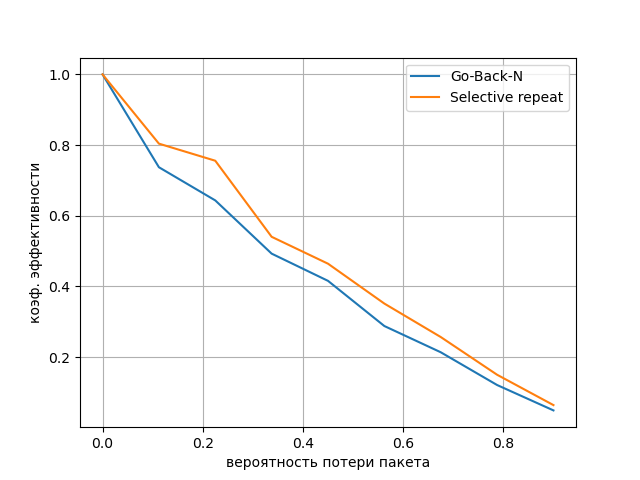
\includegraphics[scale=0.5]{fig1}
		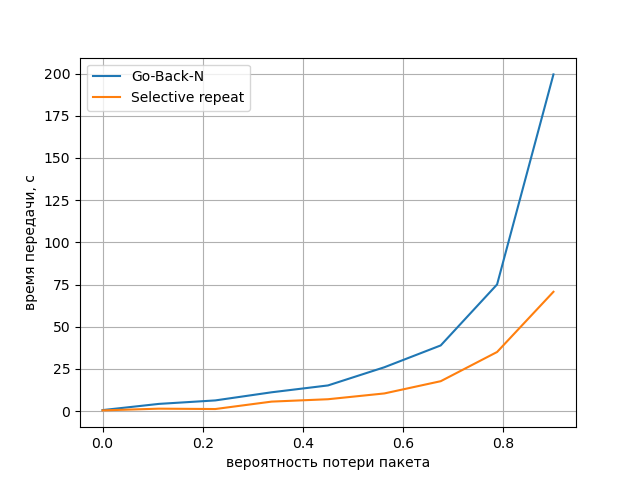
\includegraphics[scale=0.5]{fig2}
		\caption{Визуализация передачи данных с использованием скользящего окна}
	\end{center}
\end{figure}

\begin{table}[H]
	\begin{center}
		\begin{tabular}{|c|c|c|c|c|}
			\hline
			 & \multicolumn{2}{c|}{Go-Back-N} & \multicolumn{2}{c|}{Selective Repeat} \\
			\hline
			$p$ & $k$ & $t$ & $k$ & $t$ \\
			\hline
			0.0 & 0.55 & 1.00 & 0.37 & 1.00 \\
			\hline
			0.1 & 4.23 & 0.74 & 1.40 & 0.80\\
			\hline
			0.2 & 6.29 & 0.64 & 1.18 & 0.76\\
			\hline
			0.3 & 11.11 & 0.49 & 5.59 & 0.54\\
			\hline
			0.5 & 15.17 & 0.42 & 6.99 & 0.46\\
			\hline
			0.6 & 25.95 & 0.29 & 10.43 & 0.35\\
			\hline
			0.7 & 38.89 & 0.21 & 17.68 & 0.26\\
			\hline
			0.8 & 75.04 & 0.12 & 35.00 & 0.15\\
			\hline
			0.9 & 199.54 & 0.05 & 70.68 & 0.06\\
			\hline
		\end{tabular}
		\caption{ Зависимость эффективности протоколов от вероятности потери пакета при window\_size = 3}
	\end{center}
\end{table}


Зависимость
эффективности $k$ и времени передачи $t$ от размера окна window\_size при
заданной вероятности потери пакета $p = 0.3$ представлена в табл. 2 и на рис. 5.

\begin{figure}[H]
	\begin{center}
		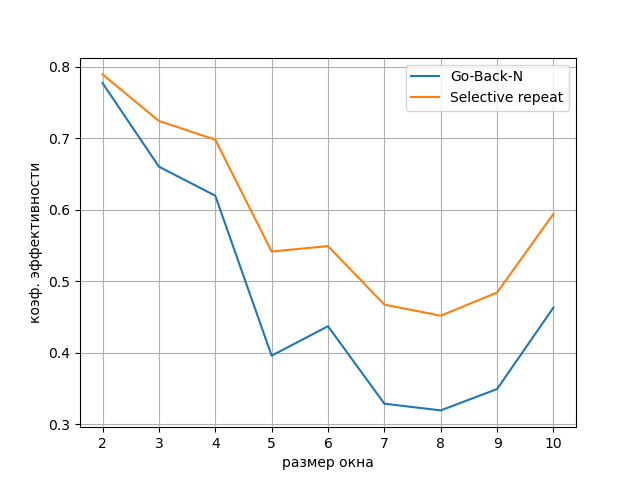
\includegraphics[scale=0.52]{fig3}
		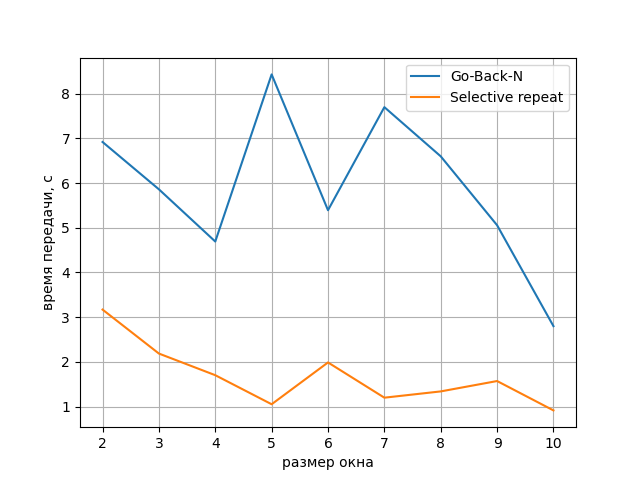
\includegraphics[scale=0.52]{fig4}
		\caption{Зависимость коэффициента эффективности и времени передачи от размера окна при $p = 0.3$}
	\end{center}
\end{figure}

\begin{table}[H]
	\begin{center}
		\begin{tabular}{|c|c|c|c|c|}
			\hline
			& \multicolumn{2}{c|}{Go-Back-N} & \multicolumn{2}{c|}{Selective Repeat} \\
			\hline
			window size & $k$ & $t$ & $k$ & $t$ \\
			\hline
			2 & 6.92 & 0.78 & 3.17 & 0.79 \\
			\hline
			3 & 5.86 & 0.66 & 2.19 & 0.72\\
			\hline
			4 & 4.69 & 0.62 & 1.70 & 0.70\\
			\hline
			5 & 8.43 & 0.40 & 1.05 & 0.54\\
			\hline
			6 & 5.39 & 0.44 & 1.99 & 0.55\\
			\hline
			7 & 7.70 & 0.33 & 1.20 & 0.47\\
			\hline
			8 & 6.60 & 0.32 & 1.34 & 0.45\\
			\hline
			9 & 5.06 & 0.35 & 1.57 & 0.48\\
			\hline
			10 & 2.80 & 0.46 & 0.91 & 0.59\\
			\hline
		\end{tabular}
		\caption{Зависимость эффективности протоколов от вероятности потери пакета при window\_size = 3}
	\end{center}
\end{table}
